t\section{روش‌های مبتنی بر مدل کدگذار-کدگشا}
با پیشرفت‌های اخیر در پردازش زبان طبیعی، مدل‌های کدگذار-کدگشا به‌عنوان یکی از رویکردهای مؤثر در وظایف تولید متن، از جمله ترجمه ماشینی و خلاصه‌سازی متن، مطرح شده‌اند. این مدل‌ها با نگاشت ورودی به خروجی، امکان تولید نتایج مطلوب را فراهم می‌کنند. معماری کدگذار-کدگشا، که در شکل \ref{fig:encoder_decoder} نمایش داده شده است، اساس مدل‌های دنباله به دنباله را تشکیل می‌دهد.

در این ساختار، کدگذار وظیفه دارد ورودی‌ها را به یک نمایش داخلی تبدیل کند، در حالی که کدگشا از این نمایش داخلی برای تولید خروجی‌ها استفاده می‌کند. هر دو بخش از مکانیزم توجه بهره می‌برند که به مدل اجازه می‌دهد تمرکز خود را بر روی بخش‌های مهم‌تر ورودی یا خروجی تنظیم کند. 

شبکه‌های عصبی بازگشتی \LTRfootnote{RNN} و حافظه‌های کوتاه‌مدت طولانی \LTRfootnote{LSTM} برای پردازش داده‌های دنباله‌ای مانند متن طراحی شده‌اند و در این زمینه عملکرد مناسبی دارند. با این حال، این مدل‌ها در مدیریت وابستگی‌های طولانی‌مدت با چالش‌هایی مواجه هستند. برای غلبه بر این محدودیت‌ها، مدل‌های ترنسفورمر معرفی شدند که با استفاده از مکانیزم توجه، امکان پردازش موازی و مدیریت وابستگی‌های دوربرد را فراهم می‌کنند. در ادامه، به بررسی مدل‌های کدگذار-کدگشا و نقش آن‌ها در پیشرفت‌های اخیر پردازش زبان طبیعی می‌پردازیم. 
%قبل از ظهور ترنسفورمرها، مدل‌های شبکه عصبی عمیق دنباله به دنباله  بهترین مدل برای وظایف تولید متن از جمله ترجمه‌ی ماشینی و خلاصه‌سازی متن بوده‌اند. این مدل‌ها ورودی را از یک فرم به فرم دیگر نگاشت می‌کنند تا نتایج مورد نظر را تولید کنند. معماری کدگذار-کدگشا رویکرد اصلی برای مدل‌سازی مدل‌های دنباله به دنباله است. شکل\ref{fig:encoder_decoder} معماری پایه‌‌ی مدل کدگذار-کدگشا را شرح می‌دهد.شبکه‌های عصبی بازگشتی\LTRfootnote{recurrent neural network (RNN)}
%\cite{elman1990finding}
%و حافظه‌های کوتاه مدت طولانی\LTRfootnote{long short-term memory networks(LSTM)} \cite{hochreiter1997long}برای توالی طراحی شده‌اند و برای کدگذاری و پردازش داده‌های دنباله‌ای مانند متن مناسب هستند اما در مدیریت حافظه‌ی بلند مدت مشکل دارند.
\begin{figure}[!h]
	\begin{center}
		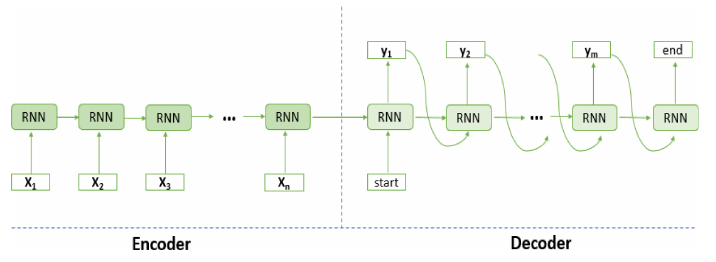
\includegraphics[height=6cm]{encoder_decoder.png}
	\end{center}
	\caption{معماری پایه‌‌ی مدل کدگذار-کدگشا \cite{RL_survey}}
	\label{fig:encoder_decoder}
	\medskip
	\small
\end{figure}

یائو\LTRfootnote{Yao}
و همکاران مدل کدگذاری دوگانه را برای خلاصه‌سازی انتزاعی پیشنهاد داده‌اند. این مدل برای درک بهتر روابط بین متن ورودی و خلاصه مرجع بازنمایی متن ورودی و بازنمایی خلاصه‌ی مرجع را می‌آموزد. همانطور که در شکل \ref{fig:dual_encoder} نشان داده شده است.
%کدگذاری دوگانه به مدل اجازه می‌دهد تا دو نمایش متفاوت از متن را بیاموزد: نمایش متن ورودی و نمایش خلاصه مرجع. این به مدل اجازه می‌دهد تا روابط بین متن ورودی و خلاصه مرجع را بهتر درک کند، که می‌تواند منجر به خلاصه‌های دقیق‌ و حاوی اطلاعات مفید شود.
این مدل از یک کدگذار اولیه، یک کدگذار ثانویه و یک کدگشا مجهز به مکانیزم توجه تشکیل شده است و هر سه ماژول فوق از واحد بازگشتی دروازه‌ای
\LTRfootnote{gated recurrent unit (GRU)}
استفاده می‌کنند. 
کدگذار اولیه بردارهای معنایی هر کلمه در ترتیب ورودی را محاسبه می‌کند. کدگذار ثانویه وزن اهمیت هر کلمه در ترتیب ورودی و بردارهای معنایی مربوطه را دوباره محاسبه می‌کند. در نهایت کدگشا با مکانیسم توجه به صورت مرحله‌ای کدگشایی می‌کند و در هر مرحله یک توالی خروجی با طول ثابت جزئی ایجاد می‌کند. در این مدل کدگذار ثانویه عملیات کدگذاری را براساس ورودی هر مرحله و خروجی مرحله‌ی قبل انجام می‌دهد بنابراین کیفیت متون قبلی تولید شده توسط کدگشا بر خروجی‌های جدید تاثیر می‌گذارد
\cite{yao2018dual}.



\begin{figure}[!h]
	\begin{center}
		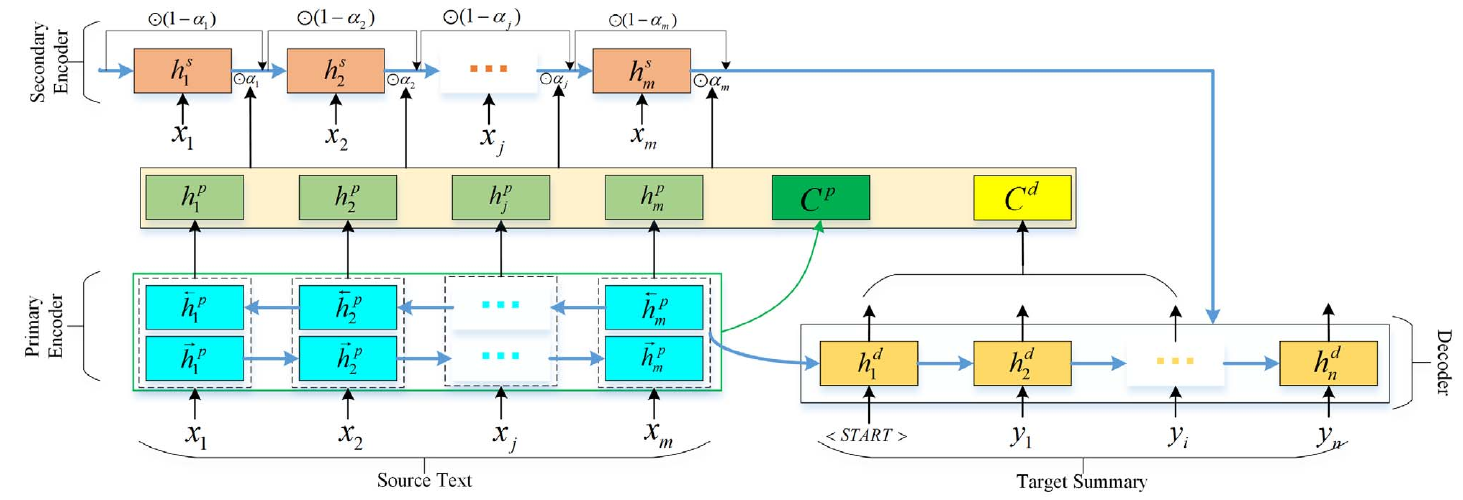
\includegraphics[height=5cm]{dualـencoder.png}
	\end{center}
	\caption{معماری پایه‌‌ی مدل دوگانه‌ی کدگذار 	 \cite{yao2018dual}}
	\label{fig:dual_encoder}
	\medskip
	\small
\end{figure}


مدل کدگذاری دوگانه مدل سلسله مراتبی متغیر بر اساس مدل کدگذاری دوگانه برای خلاصه‌سازی متقاطع زبانی\LTRfootnote{cross-lingual}
پیشنهاد شده است. این مدل شامل دو متغیر نهفته محلی و یک متغیر نهفته جامع است. از متغیرهای نهفته محلی برای بازسازی ترجمه و خلاصه زبان مبدأ و از متغیر نهفته سراسری برای تولید خلاصه بین زبانی استفاده می‌شود. قسمت کد گذار این مدل دو بخش دارد که هر بخش وظیفه‌ی تولید یکی از متغیرهای نهفته محلی را دارد و بخش کدگشا با استفاده از نمایش‌های نهفته‌ی محلی خلاصه‌ی نهایی را تولید می‌کند.
ساختار سلسله مراتبی این مدل به آن اجازه می‌دهد تا رابطه سلسله مراتبی بین ترجمه، خلاصه‌سازی و خلاصه‌سازی بین زبانی را بیاموزد \cite{variational}.

\begin{figure}[!h]
	\begin{center}
		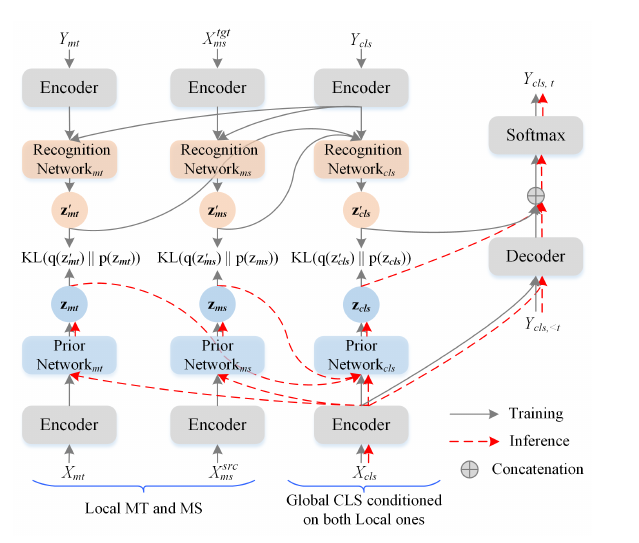
\includegraphics[height=12cm]{Variational Hierarchical Model.png}
	\end{center}
	\caption{معماری پایه‌‌ی مدل سلسله مراتبی متغیر برای خلاصه‌سازی متقابل زبانی \cite{variational}}
	\label{fig:vahie_model}
	\medskip
	\small{
		متغیرهای محلی $ z_mt $ و $ z_ms $ به ترتیب برای ترجمه و خلاصه‌سازی و متغیر جامع $ z_cls $ برای خلاصه‌سازی بین زبانی طراحی شده‌اند. خطوط خاکستری نشان‌دهنده فرآیند آموزشی است که مسئول تولید
		($ z' _{mt} $، $ z'_{ms} $، $ z'_{cls} $)
		از توزیع پسین متناظر پیش‌بینی‌شده توسط شبکه‌ است. خطوط قرمز خط چین نشان دهنده فرآیند استنتاج برای تولید نمایش‌‌های نهفته
		($ z _{mt} $، $ z_{ms} $، $ z_{cls} $)
		از توزیع‌های پیش بینی شده توسط شبکه‌های قبلی است. }
\end{figure}
